\documentclass[paper=a5,DIV=15,headinclude,twoside=semi,openany,titlepage=firstiscover]{scrbook}
\usepackage[utf8]{inputenc}
\usepackage[T1]{fontenc}
\usepackage[swedish]{babel}
\usepackage{lipsum}
\title{En liten guide för att skriva fallrapport}
\author{T. Tolvansson}
\date{October 2020}
\usepackage{calc}
\usepackage[dvipsnames]{xcolor}
\usepackage{tikz}
\usetikzlibrary{shapes}
\usetikzlibrary{calc}
\usepackage{anyfontsize}
%\usepackage{sectsty}
\usepackage[lf]{linguisticspro}
\usepackage{Rosario}
\usepackage{paralist}
\usepackage{array}
\usepackage{xhfill}
\usepackage{ragged2e}
\lowertitleback{%
test text

}
\newcommand{\siffergrey}{black!50!white}

%\newcommand{\sifferlinje}[1]{%
%	\noindent\textcolor{black!50!white}{{\huge  \textcolor{\siffergrey}{#1}}\xrfill[.5ex]{2pt}[\siffergrey]}}
%}

\newcommand{\sifferlinje}[1]{%
	\noindent{\large\textcolor{black}{#1}}\xrfill[0ex]{1pt}
}

\begin{document}
\frontmatter
\begin{titlepage}
\begin{tikzpicture}[remember picture,overlay]
%\fill[BlueViolet] (current page.south west) rectangle (current page.north east);
%%% NEDRE VÄNSTER
\begin{scope}
\foreach \i in {2.5,...,15.5}
{\node[rounded corners,black!30,draw,regular polygon,regular polygon sides=6, minimum size=\i cm,ultra thick] at ($(current page.west)+(2.5,-5)$) {} ;}
\end{scope}

%%% ÅR
%\node[rounded corners,text=black!60,regular polygon,regular polygon sides=6, minimum size=2.5 cm,inner sep=0,ultra thick] at ($(current page.west)+(2.5,-5)$) {\LARGE \bfseries 2020};

\node (myfirstpic) at ($(current page.west)+(2.5,-5)$) {
\includegraphics[scale=0.12]{coverfallrisksymbol}};

%%% Uppe vänster
\foreach \i in {0.5,...,18}
{\node[rounded corners,black!30,draw,regular polygon,regular polygon sides=6, minimum size=\i cm,ultra thick] at ($(current page.north west)+(2.5,0)$) {} ;}

%%% Höger uppe
\foreach \i in {0.5,...,15}
{\node[rounded corners,black!10,draw,regular polygon,regular polygon sides=6, minimum size=\i cm,ultra thick] at ($(current page.north east)+(0,-9.5)$) {} ;}

%%% nere höger centrum
%\foreach \i in {5}
%{\node[rounded corners,draw=black!70,regular polygon,regular polygon sides=6, minimum size=\i cm,ultra thick] at ($(current page.south east)+(-0.2,-0.45)$) {} ;}

%%% nere höger hexagon
\foreach \i in {12,...,0.5}
{\node[black!20,rounded corners,draw,regular polygon,regular polygon sides=6, minimum size=\i cm,ultra thick] at ($(current page.south east)+(-0.2,-0.45)$) {} ;}

%%% TEXTER


%%% 
%\node[left,black,minimum width=0.625*\paperwidth,minimum height=2cm, rounded corners] at ($(current page.north east)+(-2,-11)$){{\huge \textit{Subtitle of the Report}}};

\node[black,minimum width=0.625*\paperwidth,minimum height=2cm, rounded corners] at ($(current page.north east)+(-4,-7)$){{\LARGE \textit{En liten guide till}}};

\node[black,minimum width=0.625*\paperwidth,minimum height=3cm, rounded corners] at ($(current page.north east)+(-5,-8.25)$){{\fontsize{25}{30} \selectfont \bfseries att skriva fallrapporter}};

\end{tikzpicture}
\end{titlepage}

\mainmatter
\pagestyle{empty}

\section*{När ska en fallrapport skrivas?}
\textit{Varje gång en brukare oavsiktligen hamnar på golvet}. Det kan vara att tappa balansen och trilla, men också att glida ur sängen eller att benen viker sig när man reser sig från toaletten. Om brukaren hamnar på golvet, och det inte var avsiktligt, ska en fallrapport skrivas.

\section*{Vad ska jag göra efter en fallhändelse?}
\begin{itemize}
	\item Kontakta sjuksköterska.
	\item Dokumentera fallhändelsen i Procapita.
\end{itemize}
Om du är med en brukare som precis har fallit, ta det lugnt. Stressa inte upp dig. Prata lugnt med brukaren. Om du inte såg vad som hände så kan det vara bra att vara extra försiktig. Ser det ut som att brukaren har slagit i huvudet? Be brukaren att röra på armar och ben. Vid huvudskada eller misstänkt fraktur, vänta på sjuksköterska. Lägg en kudde under huvudet och gör det bekvämt för brukaren. Golv kan vara kalla, så en filt kan kännas bra med. Om ni är två så är det bra om en stannar med brukaren så att han/hon känner sig trygg.

\clearpage

%\begin{enumerate}
%    \item Klicka på ”Komponenter” i navigeringsfliken.\\ 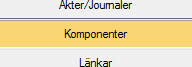
\includegraphics{fall1}
%    \item Dubbelklicka på ”Avvikelser”\\ 
\includegraphics{fall2}
%    \item Fyll i personnummer och klika på ikonen ”kikare”
%    \item Klicka på ikonen ”ny”
%    5\item Kontrollera att organisationen stämmer
%    \item Välj avvikelse ”HSL - Fallhändelse” i rull-listan.
%    \item Välj mottagare ”Vevrehemmet Äbo - HSL” eller ”Vevrehemmet Dembo - HSL”
%    \item Fyll i all information nedan. ”Pågick till” och ”Medanmälare” är frivilligt. Obs! Händelsedatum och -tid anger när fallet inträffade, inte när det upptäcktes.
%    \item Klicka på fliken ”Ytterligare uppgifter”
%    10\item Fyll i all information nedan förutom ”Allvarlighetsgrad”.
%    \item Klicka på ikonen ”Spara”.
%    \item Klicka på fliken ”Dokumentation”
%    \item Öppna ”Avvikelse HSL” och dokumentera under ”Beskrivning av händelseförloppet.” (Läs mer om detta på nästa sida.)
%    \item Klicka på ikonen ”Spara”.
%    \item Signera när rutan för signering kommer upp på skärmen.
%\end{enumerate}

\section*{Steg för steg i Procapita}

%\sifferlinje{1}
%\indent \hrulefill
\noindent\hrulefill
%%% 1.
\vfill
\noindent
\begin{minipage}[t]{0.06\textwidth}
\phantom{1}1.
\end{minipage}%
\begin{minipage}[t]{.49\textwidth}\raggedright
Klicka på ``\textbf{Komponenter}'' i\\ navigeringsfliken.
\end{minipage}% This must go next to `\end{minipage}`
\begin{minipage}[t]{.45\textwidth}
\hfill\raisebox{-\height+0.7\baselineskip}{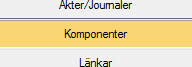
\includegraphics[scale=1]{fall1}}
\end{minipage}
\vfill

\noindent\hrulefill

%%% 2
\vfill
\noindent
\begin{minipage}[t]{0.06\textwidth}
\phantom{1}2.
\end{minipage}%
\begin{minipage}[t]{.49\textwidth}\raggedright
	Dubbelklicka på ``\textbf{Avvikelser}''.
\end{minipage}%
\begin{minipage}[t]{.45\textwidth}
	\hfill\raisebox{-\height+0.7\baselineskip}{
\includegraphics[scale=1]{fall2}}
\end{minipage}
\vfill

\noindent\hrulefill

%%% 3
\vfill
\noindent
\begin{minipage}[t]{0.06\textwidth}
	\phantom{1}3.
\end{minipage}%
\begin{minipage}[t]{.44\textwidth}\raggedright
	Fyll i personnummer och\\ klicka på ikonen ``\textbf{kikare}''.
\end{minipage}% This must go next to `\end{minipage}`
\begin{minipage}[t]{.5\textwidth}
	\hfill\raisebox{-\height+0.7\baselineskip}{
\includegraphics[scale=1]{fall3}}
\end{minipage}
\vfill

\noindent\hrulefill

%%% 4
\vfill
\noindent
\begin{minipage}[t]{0.06\textwidth}
	\phantom{1}4.
\end{minipage}%
\begin{minipage}[t]{.44\textwidth}\raggedright
	Klicka på ikonen ``\textbf{ny}''\\(ett vitt ark uppe till vänster).
\end{minipage}% This must go next to `\end{minipage}`
\begin{minipage}[t]{.5\textwidth}
	\hfill\raisebox{-\height+0.7\baselineskip}{
\includegraphics[scale=1]{fall4}}
\end{minipage}
\vfill

\noindent\hrulefill

%%% 5
\vfill
\noindent
\begin{minipage}[t]{0.06\textwidth}
	\phantom{1}5.
\end{minipage}%
\begin{minipage}[t]{.44\textwidth}\raggedright
	Kontrollera att \textbf{organisationen} stämmer.
\end{minipage}% This must go next to `\end{minipage}`
\begin{minipage}[t]{.5\textwidth}
	\hfill\raisebox{-\height+0.7\baselineskip}{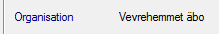
\includegraphics[scale=0.9]{fall5}}
\end{minipage}
\vfill

\noindent\hrulefill

%%% 6
\vfill
\noindent
\begin{minipage}[t]{0.06\textwidth}
	\phantom{1}6.
\end{minipage}%
\begin{minipage}[t]{.54\textwidth}\raggedright
	Välj \textbf{avvikelse} ”HSL - Fallhändelse”\\
	i rull-listan.
\end{minipage}% This must go next to `\end{minipage}`
\begin{minipage}[t]{.4\textwidth}
	\hfill\raisebox{-\height+0.7\baselineskip}{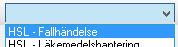
\includegraphics[scale=1]{fall6a}}
\end{minipage}
\vfill

\noindent\hrulefill

%%% 7
\vfill
\noindent
\begin{minipage}[t]{0.06\textwidth}
	\phantom{1}7.
\end{minipage}%
\begin{minipage}[t]{.54\textwidth}\raggedright
	Välj \textbf{mottagare}:\\ 
	”Vevrehemmet Dembo - HSL” eller\\”Vevrehemmet Äbo - HSL”
\end{minipage}% This must go next to `\end{minipage}`
\begin{minipage}[t]{.4\textwidth}
	\hfill\raisebox{-\height+0.7\baselineskip}{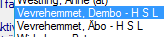
\includegraphics[scale=1.05]{fall7a}}
\end{minipage}
\vfill

\noindent\hrulefill
\newpage
\noindent\hrulefill

%%% 8
\vfill
\noindent
\begin{minipage}[t]{0.06\textwidth}
	\phantom{1}8.
\end{minipage}%
\begin{minipage}[t]{.94\textwidth}\raggedright
	\textbf{Fyll i} all information på denna sida. ”Pågick till” och ”Medanmälare” är frivilligt. \textit{OBS! ``Har hemvård'' ska fyllas i ``Ja''}.
\end{minipage}% This must go next to `\end{minipage}`
%\begin{minipage}[t]{.4\textwidth}
%	\hfill\raisebox{-\height+0.7\baselineskip}{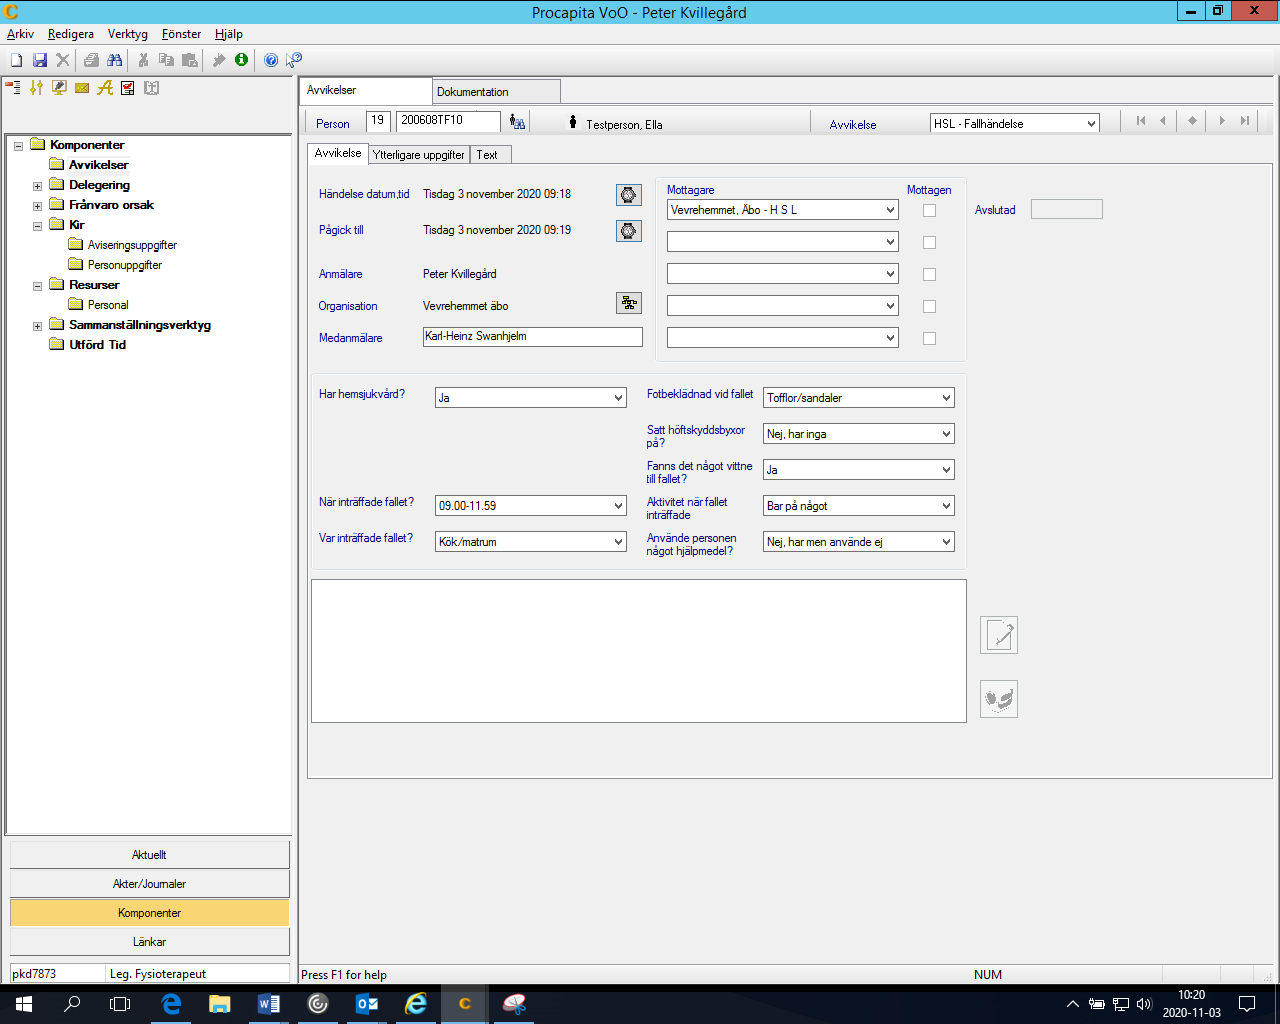
\includegraphics[scale=1.1]{fall8}}
%\end{minipage}
\vfill

\noindent\hrulefill

%%% 9
\vfill
\noindent
\begin{minipage}[t]{0.06\textwidth}
	\phantom{1}9.
\end{minipage}%
\begin{minipage}[t]{.54\textwidth}\raggedright
	Klicka på fliken\\”\textbf{Ytterligare uppgifter}”.
\end{minipage}% This must go next to `\end{minipage}`
\begin{minipage}[t]{.4\textwidth}
	\hfill\raisebox{-\height+0.7\baselineskip}{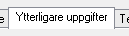
\includegraphics[scale=1]{fall9a}}
\end{minipage}
\vfill

\noindent\hrulefill

%%% 10
\vfill
\noindent
\begin{minipage}[t]{0.06\textwidth}
	10.
\end{minipage}%
\begin{minipage}[t]{.94\textwidth}\raggedright
	\textbf{Fyll i} all information för ``Ytterligare uppgifter'' förutom\\ ”Allvarlighetsgrad”. \textit{OBS! Fyll inte i ``Allvarlighetsgrad''}.
\end{minipage}% This must go next to `\end{minipage}`
%\begin{minipage}[t]{.4\textwidth}
%	\hfill\raisebox{-\height+0.7\baselineskip}{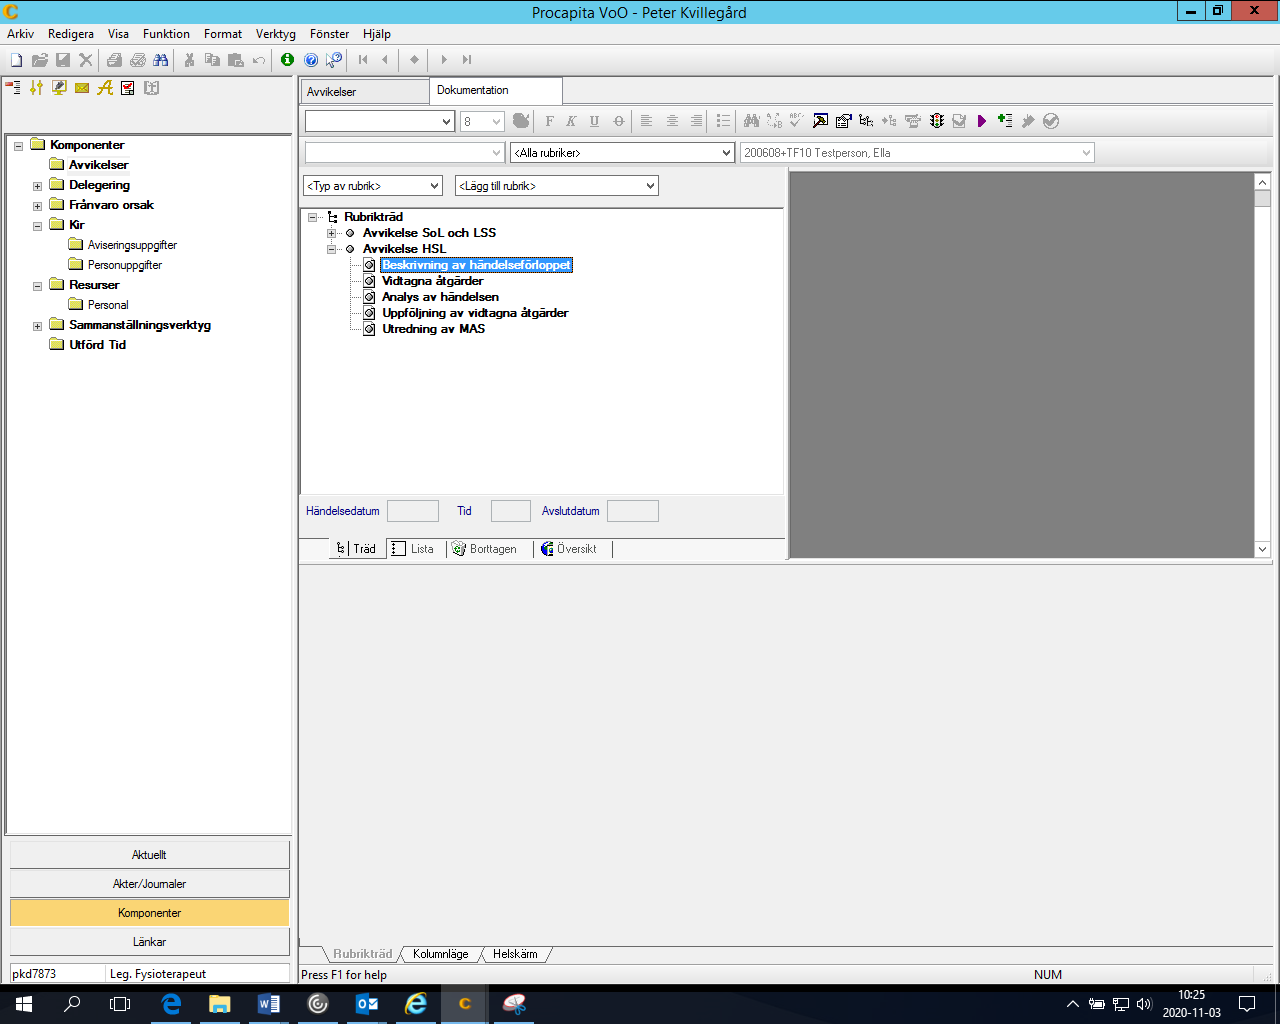
\includegraphics[scale=1]{fall10}}
%\end{minipage}
\vfill

\noindent\hrulefill

%%% 11
\vfill
\noindent
\begin{minipage}[t]{0.06\textwidth}
	11.
\end{minipage}%
\begin{minipage}[t]{.44\textwidth}\raggedright
	Klicka på ikonen ”\textbf{Spara}”.
\end{minipage}% This must go next to `\end{minipage}`
\begin{minipage}[t]{.5\textwidth}
	\hfill\raisebox{-\height+0.7\baselineskip}{
\includegraphics[scale=1]{fall11a}}
\end{minipage}
\vfill

\noindent\hrulefill

%%% 12
\vfill
\noindent
\begin{minipage}[t]{0.06\textwidth}
	12.
\end{minipage}%
\begin{minipage}[t]{.44\textwidth}\raggedright
	Klicka på fliken ”\textbf{Dokumentation}”.
\end{minipage}% This must go next to `\end{minipage}`
\begin{minipage}[t]{.5\textwidth}
	\hfill\raisebox{-\height+0.7\baselineskip}{
\includegraphics[scale=1]{fall12}}
\end{minipage}
\vfill

\noindent\hrulefill

%%% 13
\vfill
\noindent
\begin{minipage}[t]{0.06\textwidth}
	13.
\end{minipage}%
\begin{minipage}[t]{.45\textwidth}\raggedright
	Öppna ”\textbf{Avvikelse HSL}” och dokumentera under ”\textbf{Beskrivning av händelseförloppet}”. (Läs mer om detta på nästa sida.)
\end{minipage}% This must go next to `\end{minipage}`
\begin{minipage}[t]{.49\textwidth}
	\hfill\raisebox{-\height+0.7\baselineskip}{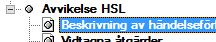
\includegraphics[scale=1]{fall13}}
\end{minipage}
\vfill

\noindent\hrulefill

%%% 14
\vfill
\noindent
\begin{minipage}[t]{0.06\textwidth}
	14.
\end{minipage}%
\begin{minipage}[t]{.44\textwidth}\raggedright
	Klicka på ikonen ”\textbf{Spara}”.
\end{minipage}% This must go next to `\end{minipage}`
\begin{minipage}[t]{.5\textwidth}
	\hfill\raisebox{-\height+0.7\baselineskip}{
\includegraphics[scale=1]{fall11a}}
\end{minipage}
\vfill

\noindent\hrulefill

%%% 15
\vfill
\noindent
\begin{minipage}[t]{0.06\textwidth}
	15.
\end{minipage}%
\begin{minipage}[t]{.44\textwidth}\raggedright
	\textbf{Signera} när rutan för signering kommer upp på skärmen.
\end{minipage}% This must go next to `\end{minipage}`
\begin{minipage}[t]{.5\textwidth}
	\hfill\raisebox{-\height+0.7\baselineskip}{
\includegraphics[scale=1]{fall15}}
\end{minipage}
\vfill

\noindent\hrulefill

\clearpage
\justify
\section*{Att beskriva händelseförloppet}
En beskrivning bör innehålla själva händelsen, men det finns fler saker som kan vara bra att få med, exempelvis:
\begin{itemize}
	\item Hur upptäcktes fallet?
	\item Vad gjorde brukaren vid falltillfället?
	\item Symtom före fallet?
	\item Omständigheter i omgivningen (Exempelvis belysning, möblering, mm.)
	\item Om brukaren vanligtvis använder hjälpmedel, användes det vid falltillfället, eller var fanns det?
	\item Uppgav brukaren någon smärta?
	\item Sa brukaren något om vad som hänt?
\end{itemize}

\subsection*{Exempel på beskrivning av händelseförloppet}

{\itshape
	Brukaren larmade själv kl 06:30, personal gick direkt till lägenheten och hittade brukaren sittandes på golvet utanför toaletten. 
	
	\noindent Hon verkar ha varit på väg gåendes till toaletten. 
	
	\noindent Hon har varit vaken stora delar av natten och verkat lite konfusorisk, men inte uppgett någon smärta. 
	
	\noindent Lamporna i rummet var släckta. Inga hinder fanns i hennes väg.
	
	\noindent Vanligtvis använder brukaren rollator vid förflyttningar i rummet, men vid detta tillfälle stod den vid sängen med låsta bromsar. 
	
	\noindent Hon uppgav att det inte gjorde ont någonstans. 
	
	\noindent Brukaren uppgav att hon behövt gå på toaletten och använt möbler som stöd när hon gick, men att hon inte fått ett bra grepp om något.
}

\clearpage

\begin{center}
\vspace*{\stretch{0.66}}
\Huge\textit{Kom ihåg!}\Large\\[2ex]

``Har hemsjukvård?'' -- ``Ja''\\[2ex]

Fyll \textbf{inte} i allvarlighetsgrad.
\vspace*{\stretch{0.33}}
\end{center}%
\end{document}


